\documentclass{article}
\usepackage[utf8]{inputenc}
\usepackage{amsmath}
\usepackage{geometry}
\usepackage{enumitem}
\usepackage{tikz}
\usetikzlibrary{shapes,arrows,positioning,calc}

\geometry{a4paper, margin=1in}

\title{\textbf{Neural Network Solutions: Past Paper}}
\author{Solution Guide}
\date{\today}

\begin{document}

\maketitle

\section*{Question 8: Neural Network Calculation}

\subsection*{Given Data}
\begin{itemize}
    \item \textbf{Inputs:} $O_1 = 0.4$, $O_2 = 0.6$
    \item \textbf{Target Output:} $T = 0.65$
    \item \textbf{Learning Rate:} $r = 0.5$
    \item \textbf{Initial Weights:}
    \begin{itemize}
        \item $w_{1i} = 0.20, w_{1j} = 0.10, w_{1k} = 0.30$
        \item $w_{2i} = -0.10, w_{2j} = -0.10, w_{2k} = 0.20$
        \item $w_{ix} = 0.10, w_{jx} = 0.50, w_{kx} = 0.20$
    \end{itemize}
    \item \textbf{Activation Function:} Sigmoid $f(x) = \frac{1}{1 + e^{-x}}$
\end{itemize}

\subsection*{Network Architecture}
\begin{center}
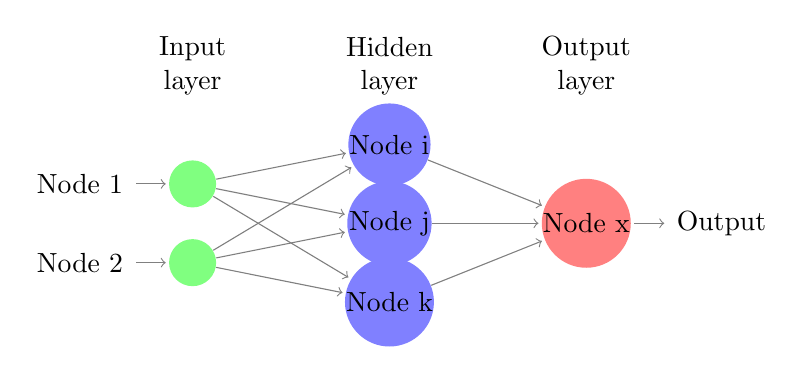
\begin{tikzpicture}[shorten >=1pt,->,draw=black!50, node distance=2.5cm]
    \tikzstyle{every pin edge}=[<-,shorten <=1pt]
    \tikzstyle{neuron}=[circle,fill=black!25,minimum size=17pt,inner sep=0pt]
    \tikzstyle{input neuron}=[neuron, fill=green!50];
    \tikzstyle{output neuron}=[neuron, fill=red!50];
    \tikzstyle{hidden neuron}=[neuron, fill=blue!50];
    \tikzstyle{annot} = [text width=4em, text centered]

    % Draw the input layer nodes
    \foreach \name / \y in {1/1, 2/2}
        \node[input neuron, pin=left:Node \name] (I-\name) at (0,-\y) {};

    % Draw the hidden layer nodes
    \foreach \name / \y in {i/0.5, j/1.5, k/2.5}
        \node[hidden neuron] (H-\name) at (2.5cm,-\y) {Node \name};

    % Draw the output layer node
    \node[output neuron,pin={[pin edge={->}]right:Output}] (O) at (5cm,-1.5) {Node x};

    % Connect every node in input layer with every node in hidden layer
    \foreach \source in {1,2}
        \foreach \dest in {i,j,k}
            \path (I-\source) edge (H-\dest);

    % Connect every node in hidden layer with the output layer
    \foreach \source in {i,j,k}
        \path (H-\source) edge (O);

    % Annotate the layers
    \node[annot,above of=H-i, node distance=1cm] (hl) {Hidden layer};
    \node[annot,left of=hl] {Input layer};
    \node[annot,right of=hl] {Output layer};
\end{tikzpicture}
\end{center}

\subsection*{Step-by-Step Calculation}

\subsubsection*{1. Hidden Layer - Net Input and Output}
For each hidden node $i, j, k$:
\begin{align*}
    net_i &= (w_{1i} \cdot O_1) + (w_{2i} \cdot O_2) = (0.20 \cdot 0.4) + (-0.10 \cdot 0.6) = 0.08 - 0.06 = 0.02000 \\
    O_i &= f(0.02000) = \frac{1}{1 + e^{-0.02}} \approx 0.50500 \\
    \\
    net_j &= (w_{1j} \cdot O_1) + (w_{2j} \cdot O_2) = (0.10 \cdot 0.4) + (-0.10 \cdot 0.6) = 0.04 - 0.06 = -0.02000 \\
    O_j &= f(-0.02000) = \frac{1}{1 + e^{0.02}} \approx 0.49500 \\
    \\
    net_k &= (w_{1k} \cdot O_1) + (w_{2k} \cdot O_2) = (0.30 \cdot 0.4) + (0.20 \cdot 0.6) = 0.12 + 0.12 = 0.24000 \\
    O_k &= f(0.24000) = \frac{1}{1 + e^{-0.24}} \approx 0.55971
\end{align*}

\subsubsection*{2. Output Layer - Net Input and Output}
\begin{align*}
    net_x &= (w_{ix} \cdot O_i) + (w_{jx} \cdot O_j) + (w_{kx} \cdot O_k) \\
    net_x &= (0.10 \cdot 0.50500) + (0.50 \cdot 0.49500) + (0.20 \cdot 0.55971) \\
    net_x &= 0.05050 + 0.24750 + 0.111942 = 0.40994 \\
    O_x &= f(0.40994) = \frac{1}{1 + e^{-0.40994}} \approx 0.60107
\end{align*}

\subsubsection*{3. Error Calculation at Node x}
Using the formula $Error(x) = (T - O_x) O_x (1 - O_x)$:
\begin{align*}
    Error(x) &= (0.65 - 0.60107) \cdot 0.60107 \cdot (1 - 0.60107) \\
    Error(x) &= 0.04893 \cdot 0.60107 \cdot 0.39893 \approx 0.01173
\end{align*}

\subsubsection*{4. Weight Update for $w_{kx}$}
Using the formula $w_{ab}(new) = w_{ab}(old) + r \cdot Error(b) \cdot O_a$:
\begin{align*}
    \Delta w_{kx} &= r \cdot Error(x) \cdot O_k \\
    \Delta w_{kx} &= 0.5 \cdot 0.01173 \cdot 0.55971 \approx 0.00328 \\
    w_{kx}(new) &= 0.20 + 0.00328 = 0.20328
\end{align*}

\subsection*{Final Answers}
\begin{enumerate}
    \item \textbf{Output at node x:} $0.60107$
    \item \textbf{Error value at node x:} $0.01173$
    \item \textbf{Updated value of weight $w_{kx}$:} $0.20328$
\end{enumerate}

\pagebreak

\section*{Question 9: Generalization in Learning}

\subsection*{Part (a)}
The goal described is called \textbf{Generalization}.

\subsection*{Part (b)}
\textbf{Generalization} is the capacity of a machine learning model to perform accurately on new, previously unseen data that was not part of the training set.

\textbf{Centrality to the Learning Process:}
Generalization is the fundamental objective of machine learning because the value of a model lies in its predictive utility for real-world scenarios. A model that only performs well on its training data has likely "memorized" noise and specific instances (overfitting) rather than learning the underlying patterns and relationships. Without generalization, a model cannot be used to make decisions in the face of uncertainty or new information.

\end{document}
